\Opensolutionfile{ans}[ans/ans-0-B15-KQ]
\TNSA
\begin{ex}%[2H2V2-6]
	Một sân vận động được xây dựng theo mô hình là hình chóp cụt $OAGD.BCFE$ có hai đáy song song với nhau. Mặt sân $OAGD$ là hình chữ nhật và được gắn hệ trục $Oxyz$ như hình vẽ dưới (đơn vị trên mỗi trục tọa độ là mét). Mặt sân $OAGD$ có chiều dài $OA=100 \mathrm{~m}$, chiều rộng $OD=60 \mathrm{~m}$ và tọa độ điểm $B(10;10;8)$. Tính khoảng cách từ điểm $G$ đến mặt phẳng $(OBED)$ (kết quả làm tròn đến hàng phần chục).
	\begin{center}
	\tikzset{every picture/.style={line width=0.75pt}}         
	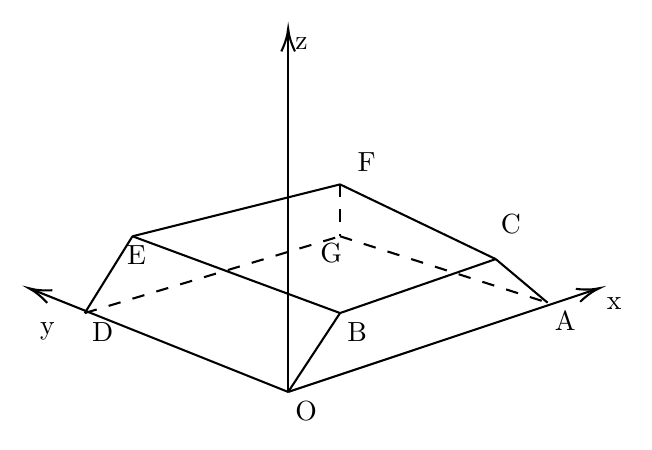
\begin{tikzpicture}[x=0.75pt,y=0.75pt,yscale=-1,xscale=1]
	\draw (250,250) -- (250,77) ;
	\draw [shift={(250,75)}, rotate = 90] [color={rgb, 255:red, 0; green, 0; blue, 0 }  ][line width=0.75]    (10.93,-3.29) .. controls (6.95,-1.4) and (3.31,-0.3) .. (0,0) .. controls (3.31,0.3) and (6.95,1.4) .. (10.93,3.29)   ;
	\draw    (250,250) -- (398.1,200.63) ;
	\draw [shift={(400,200)}, rotate = 161.57] [color={rgb, 255:red, 0; green, 0; blue, 0 }  ][line width=0.75]    (10.93,-3.29) .. controls (6.95,-1.4) and (3.31,-0.3) .. (0,0) .. controls (3.31,0.3) and (6.95,1.4) .. (10.93,3.29)   ;
	\draw    (250,250) -- (126.86,200.74) ;
	\draw [shift={(125,200)}, rotate = 21.8] [color={rgb, 255:red, 0; green, 0; blue, 0 }  ][line width=0.75]    (10.93,-3.29) .. controls (6.95,-1.4) and (3.31,-0.3) .. (0,0) .. controls (3.31,0.3) and (6.95,1.4) .. (10.93,3.29)   ;
	\draw  [dash pattern={on 4.5pt off 4.5pt}]  (152,212) -- (275,175) ;
	\draw  [dash pattern={on 4.5pt off 4.5pt}]  (275,175) -- (375,207) ;
	\draw    (175,175) -- (152,212) ;
	\draw    (175,175) -- (275,212) ;
	\draw    (250,250) -- (275,212) ;
	\draw    (275,212) -- (350,186) ;
	\draw    (350,186) -- (375,207) ;
	\draw    (175,175) -- (275,150) ;
	\draw    (275,150) -- (350,186) ;
	\draw  [dash pattern={on 4.5pt off 4.5pt}]  (275,150) -- (275,175) ;
	
	\draw (402,203) node [anchor=north west][inner sep=0.75pt]   [align=left] {x};
	
	\draw (129,215) node [anchor=north west][inner sep=0.75pt]   [align=left] {y};
	
	\draw (252,78) node [anchor=north west][inner sep=0.75pt]   [align=left] {z};
	
	\draw (252,253) node [anchor=north west][inner sep=0.75pt]   [align=left] {O};
	
	\draw (377,210) node [anchor=north west][inner sep=0.75pt]   [align=left] {A};
	
	\draw (154,215) node [anchor=north west][inner sep=0.75pt]   [align=left] {D};
	
	\draw (264,177) node [anchor=north west][inner sep=0.75pt]   [align=left] {G};
	
	\draw (177,178) node [anchor=north west][inner sep=0.75pt]   [ below] {E};
	
	\draw (277,215) node [anchor=north west][inner sep=0.75pt]   [align=left] {B};
	
	\draw (351,163) node [anchor=north west][inner sep=0.75pt]   [align=left] {C};
	
	\draw (282,133) node [anchor=north west][inner sep=0.75pt]   [align=left] {F};		
	\end{tikzpicture}
	\end{center}
\shortans{$62{,}5$}
\loigiai{Gắn hình chóp cụt $OAGD.BCFE$ vào hệ trục $Oxyz$, ta có: $O(0;0;0), A(100;0;0), G(100; 60;0), \\D(0;60;0), B(10;10;8)$, $\overrightarrow{OD}=(0 ; 60 ; 0), \overrightarrow{OB}=(10 ; 10 ; 8)$.\\
Véc-tơ pháp tuyến của mặt phẳng $(OBED)$ là $\vec{n}=[\overrightarrow{OD}, \overrightarrow{OB}]=(480 ; 0 ;-600) = 120(4 ; 0 ;-5)$.\\
Phương trình mặt phẳng $(OBED)$ đi qua điểm $O(0 ; 0 ; 0)$ và có véc-tơ pháp tuyến $\vec{n}=(4 ; 0 ;-5)$ là  $4x-5z=0$.\\
Khoảng cách từ điểm $G$ đến mặt phẳng $(OBED)$ là $$\mathrm{d}(G,(O B E D))=\dfrac{|4\cdot 100-5\cdot 0|}{\sqrt{16+25}}=\dfrac{400 \sqrt{41}}{41} \approx 62{,}5.$$
}
\end{ex}
\begin{ex}%[2H2V2-6]
	Một công trình đang xây dựng được gắn hệ trục $Oxyz$ như hình vẽ dưới (đơn vị trên mỗi trục tọa độ là mét). Mỗi cột bê tông có dạng hình lăng trụ tứ giác đều và có tâm của mặt đáy trên lần lợt là $A(3 ; 2 ; 3), B(6 ; 3 ; 3), C(9 ; 4 ; 2), D\left(6 ; 0 ; \dfrac{5}{2}\right)$. Tính khoảng cách từ điểm $D$ đến mặt phẳng $(ABC)$ (kết quả làm tròn tới hàng phần trăm).
	\begin{center}
	\includegraphics[width=0.5\linewidth]{images/h3.png}
	\end{center}
	\shortans{$2,85$}
	\loigiai{Ta có $\overrightarrow{AB}=(3;1;0); \overrightarrow{AC}=(6;2;-1)$. Phương trình mặt phẳng $(ABC)$ qua $A$ và có véc-tơ pháp tuyến $[\overrightarrow{AB},\overrightarrow{AC}]=(-1;3;0)$ là $-x + 3y - 3 = 0$. \\
	Khoảng cách từ $D$ tới mặt phẳng $(ABC)$ là $\mathrm{d}(D,(ABC))=\dfrac{\left|-6-3\right|}{\sqrt{1^2 + 3^2}}=\dfrac{9\sqrt{10}}{10} \approx 2{,}85$.
	}
\end{ex}

\begin{ex}%[2H2V2-6]
	Một công trình đang xây dựng được gắn hệ trục $Oxyz$ (đơn vị trên mỗi trục tọa độ là mét). Ba bức tường $(P),(Q),(R)$ (như hình vẽ) của tòa nhà lần lượt có phương trình $(P)\colon x+2y-2z+1=0$, $(Q)\colon 2x+y+2z-3=0,(R)\colon 2x+4y-4z-19=0$. Tính khoảng cách giữa hai bức tường $(P)$ và $(R)$ của tòa nhà.
	\begin{center}
			\includegraphics[width=0.5\linewidth]{images/h1.png}
	\end{center}
\shortans{$3{,}5$}
\loigiai{Tính khoảng cách giữa hai bức tường $(P)$ và $(R)$ của tòa nhà.\\
	Chọn điểm $M(-1 ; 0 ; 0) \in(P)$. Do hai bức tường $(P)$ và $(R)$ song song nhau nên \\
	$$\mathrm{d}((P),(R))=\mathrm{d}(M,(R))=\dfrac{|2\cdot (-1)+4\cdot 0-4\cdot 0-19|}{\sqrt{4+16+16}}=\dfrac{21}{6}=3{,}5 \text{m.}$$}
\end{ex}


\begin{ex}%[2H2V2-6]
	Một công trình đang xây dựng được gắn hệ trục $O x y z$ (đơn vị trên mỗi trục tọa độ là mét). Ba bức tường $(P),(Q),(R),(T)$ (như hình vẽ) của tòa nhà lần lượt có phương trình $(P)\colon 2x-y-z+1=0$, $(Q)\colon x+3y-z-2=0,(R)\colon 4x-2y-2 z+9=0,(T)\colon 2x+6y-2z+15=0$. Tính chiều rộng bức tường $(Q)$ của tòa nhà (kết quả làm tròn đến hàng phần chục).
	\begin{figure}[!ht]
		\centering
		\includegraphics[width=0.5\linewidth]{images/h2.png}
	\end{figure}
\shortans{$2{,}9$}
\loigiai{
	Do hai bức tường $(P)$ và $(R)$ song song nhau nên chiều rộng bức tường $(Q)$ là khoảng cách giữa hai bức tường $(P)$ và $(R)$. Chọn điểm $N(0 ; 0 ; 1) \in(P)$.\\
 Do hai bức tường $(P)$ và $(R)$ song song nhau nên $$\mathrm{d}((P),(R))=\mathrm{d}(N,(R))=\dfrac{|4\cdot 0-2\cdot 0-2\cdot 1+9|}{\sqrt{4+1+1}}=\dfrac{7}{\sqrt{6}} \approx 2{,}9.$$}
\end{ex}
\begin{ex}%[2H2V2-6]
	Cho hình lập phương $ABCD.A'B'C'D'$ có độ dài cạnh bằng 1. Gọi $M, N, P, Q$ lần lượt là trung điểm của $AB, BC, C'D',DD'$. Chọn hệ tọa độ $Oxyz$ như hình vẽ, xác định tọa độ các điểm $M, N, P, Q$. 
	Tính khoảng cách từ điểm $Q$ đến mặt phẳng $(MNP)$. Kết quả làm tròn đến hàng phần chục.
	\begin{center}
	\tikzset{every picture/.style={line width=0.75pt}} %set default line width to 0.75pt        
	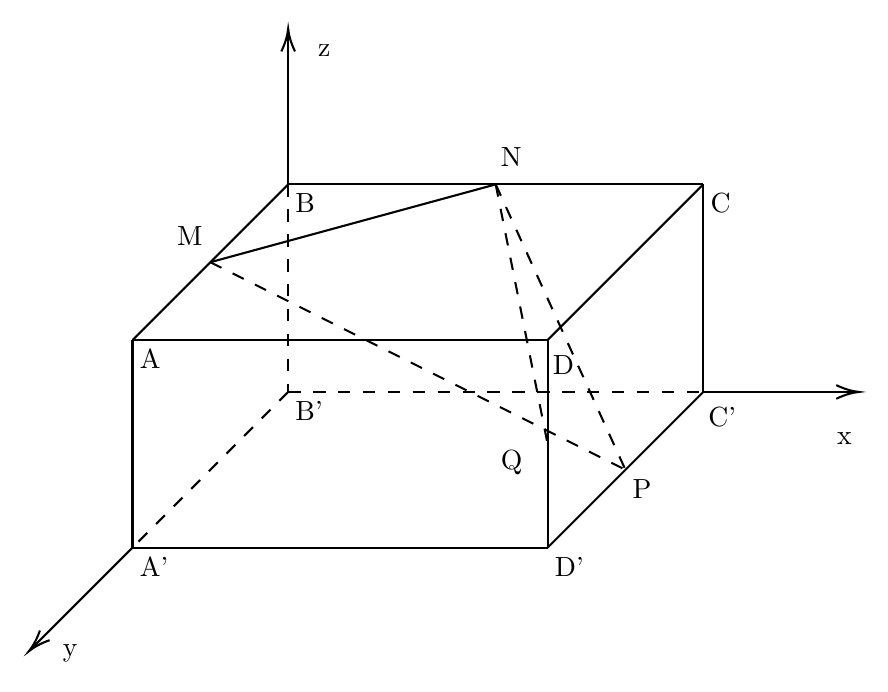
\begin{tikzpicture}[x=0.75pt,y=0.75pt,yscale=-1,xscale=1]
		%uncomment if require: \path (0,797); %set diagram left start at 0, and has height of 797
		%Straight Lines [id:da8382470567419189] 
		\draw    (250,400) -- (250,327) ;
		\draw [shift={(250,325)}, rotate = 90] [color={rgb, 255:red, 0; green, 0; blue, 0 }  ][line width=0.75]    (10.93,-3.29) .. controls (6.95,-1.4) and (3.31,-0.3) .. (0,0) .. controls (3.31,0.3) and (6.95,1.4) .. (10.93,3.29)   ;
			%Straight Lines [id:da22849660996364696] 
			\draw    (175,575) -- (375,575) ;
			%Straight Lines [id:da3429340193043935] 
			\draw    (375,575) -- (450,500) ;
			%Straight Lines [id:da6171158479105385] 
			\draw    (250,400) -- (175,475) ;
			%Straight Lines [id:da20159315767924957] 
			\draw    (175,475) -- (175,575) ;
			%Straight Lines [id:da09157475506424606] 
			\draw    (175,475) -- (375,475) ;
			%Straight Lines [id:da7794866428713987] 
			\draw    (375,475) -- (375,575) ;
			%Straight Lines [id:da5730802129402581] 
			\draw    (375,475) -- (450,400) ;
			%Straight Lines [id:da4069170044141508] 
			\draw    (250,400) -- (450,400) ;
			%Straight Lines [id:da7895384060713708] 
			\draw    (450,400) -- (450,500) ;
			%Straight Lines [id:da3822968918446086] 
			\draw    (212.5,437.5) -- (350,400) ;
			%Straight Lines [id:da5114427996681619] 
			\draw  [dash pattern={on 4.5pt off 4.5pt}]  (350,400) -- (412.5,537.5) ;
			%Straight Lines [id:da5639353335968631] 
			\draw  [dash pattern={on 4.5pt off 4.5pt}]  (212.5,437.5) -- (412.5,537.5) ;
			%Straight Lines [id:da7141193916967588] 
			\draw  [dash pattern={on 4.5pt off 4.5pt}]  (350,400) -- (375,525) ;
			%Straight Lines [id:da6592626042182406] 
			\draw  [dash pattern={on 4.5pt off 4.5pt}]  (250,500) -- (175,575) ;
			%Straight Lines [id:da4180570193860802] 
			\draw    (175,575) -- (126.41,623.59) ;
			\draw [shift={(125,625)}, rotate = 315] [color={rgb, 255:red, 0; green, 0; blue, 0 }  ][line width=0.75]    (10.93,-3.29) .. controls (6.95,-1.4) and (3.31,-0.3) .. (0,0) .. controls (3.31,0.3) and (6.95,1.4) .. (10.93,3.29)   ;
			%Straight Lines [id:da9167552187295651] 
			\draw  [dash pattern={on 4.5pt off 4.5pt}]  (250,500) -- (450,500) ;
			%Straight Lines [id:da8527980278686933] 
			\draw    (450,500) -- (523,500) ;
			\draw [shift={(525,500)}, rotate = 180] [color={rgb, 255:red, 0; green, 0; blue, 0 }  ][line width=0.75]    (10.93,-3.29) .. controls (6.95,-1.4) and (3.31,-0.3) .. (0,0) .. controls (3.31,0.3) and (6.95,1.4) .. (10.93,3.29)   ;
			%Straight Lines [id:da8000503760713495] 
			\draw  [dash pattern={on 4.5pt off 4.5pt}]  (250,400) -- (250,500) ;
			\draw (177,478) node [anchor=north west][inner sep=0.75pt]   [align=left] {A};
			
			\draw (252,403) node [anchor=north west][inner sep=0.75pt]   [align=left] {B};
			
			\draw (452,403) node [anchor=north west][inner sep=0.75pt]   [align=left] {C};
			
			\draw (376,481) node [anchor=north west][inner sep=0.75pt]   [align=left] {D};
			
			\draw (177,578) node [anchor=north west][inner sep=0.75pt]   [align=left] {A'};
			
			\draw (252,503) node [anchor=north west][inner sep=0.75pt]   [align=left] {B'};
			
			\draw (451,506) node [anchor=north west][inner sep=0.75pt]   [align=left] {C'};
			
			\draw (377,578) node [anchor=north west][inner sep=0.75pt]   [align=left] {D'};
			
			\draw (195,419) node [anchor=north west][inner sep=0.75pt]   [align=left] {M};
			
			\draw (351,381) node [anchor=north west][inner sep=0.75pt]   [align=left] {N};
			
			\draw (414.5,540.5) node [anchor=north west][inner sep=0.75pt]   [align=left] {P};
			
			\draw (351,527) node [anchor=north west][inner sep=0.75pt]   [align=left] {Q};
			
			\draw (513,518) node [anchor=north west][inner sep=0.75pt]   [align=left] {x};
			
			\draw (140,620) node [anchor=north west][inner sep=0.75pt]   [align=left] {y};
			
			\draw (263,331) node [anchor=north west][inner sep=0.75pt]   [align=left] {z};
	\end{tikzpicture}
	\end{center}
\shortans{$1,4$}
\loigiai{Thiết lập hệ tọa độ $O x y z$ như hình vẽ, gốc $O \equiv B'$. Khi đó $M\left(0 ; \dfrac{1}{2} ; 1\right), N\left(\dfrac{1}{2} ; 0 ; 1\right), P\left(1 ; \dfrac{1}{2} ; 0\right),\\
	Q\left(1 ; 1 ; \dfrac{1}{2}\right)$. Phương trình mặt phẳng $(MNP)$ đi qua $M\left(0;\dfrac{1}{2};1\right)$ và có véc-tơ pháp tuyến $[\overrightarrow {MN} ,\overrightarrow {MP}]=\left( \dfrac{1}{{2}};\dfrac{1}{{2}};\dfrac{1}{{2}}\right)$ là $2x + 2y + 2z - 3 = 0$.\\
	Khoảng cách từ điểm $Q$ đến mặt phẳng $(MNP)$ là $$\mathrm{d}(Q;(MNP)=\dfrac{\left|2\cdot 1+2\cdot 1+2\cdot \dfrac{1}{2}\right|}{\sqrt{2^2 +2^2 +2^2}}= \dfrac{5\sqrt{3}}{6}\approx 1{,}4.$$
}
\end{ex}
\begin{ex}%[2H2V2-6]
	Cho hình chóp $S.ABCD$ có đáy $ABCD$ là hình vuông cạnh $a, SAD$ là tam giác đều và nằm trong mặt phẳng với đáy. Gọi $M$ và $N$ lần lượt là trung điểm của $BC$ và $CD$. Chọn hệ tọa độ $Oxyz$ như hình vẽ dưới. Gọi $Q$ là trung điểm $S D$. Tính khoảng cách giữa hai mặt phẳng $(SAC)$ và mặt phẳng $(ONQ)$ (kết quả làm tròn đến hàng phần chục).
	\begin{center}
	% Gradient Info
	\tikzset {_0pmvymc3o/.code = {\pgfsetadditionalshadetransform{ \pgftransformshift{\pgfpoint{-198 bp } { 158.4 bp }  }  \pgftransformscale{1.32 }  }}}
		\pgfdeclareradialshading{_ffechrcqo}{\pgfpoint{160bp}{-128bp}}{rgb(0bp)=(0,0,0);
			rgb(0bp)=(0,0,0);
			rgb(6.785714285714286bp)=(0,0,0);
			rgb(14.017857142857142bp)=(0,0,0);
			rgb(20bp)=(0,0,0);
			rgb(25bp)=(1,1,1);
			rgb(400bp)=(1,1,1)}
		\tikzset{every picture/.style={line width=0.75pt}} %set default line width to 0.75pt        
	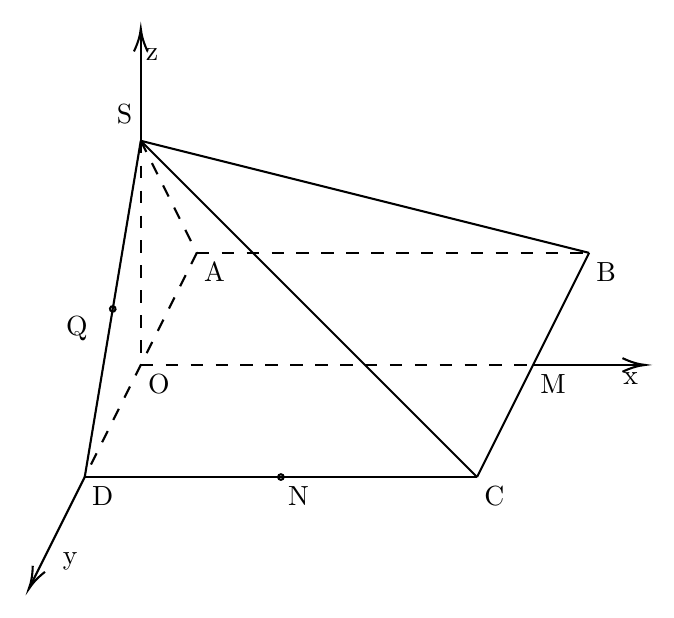
\begin{tikzpicture}[x=0.75pt,y=0.75pt,yscale=-1,xscale=1]
		%uncomment if require: \path (0,300); %set diagram left start at 0, and has height of 300
			%Straight Lines [id:da1986885226481041] 
			\draw    (108,216) -- (297,216) ;
			\draw [shift={(202.5,216)}, rotate = 0] [color={rgb, 255:red, 0; green, 0; blue, 0 }  ][line width=0.75]      (0, 0) circle [x radius= 1.34, y radius= 1.34]   ;
			%Straight Lines [id:da8495468285480916] 
			\draw [color={rgb, 255:red, 0; green, 0; blue, 0 }  ,draw opacity=1 ][shading=_ffechrcqo,_0pmvymc3o]   (135,54) -- (171,63) -- (207,72) -- (243,81) -- (279,90) -- (315,99) -- (351,108) ;
			%Straight Lines [id:da7064838767550801] 
			\draw  [dash pattern={on 4.5pt off 4.5pt}]  (135,162) -- (324,162) ;
			%Straight Lines [id:da7232875579325917] 
			\draw  [dash pattern={on 4.5pt off 4.5pt}]  (162,108) -- (108,216) ;
			%Straight Lines [id:da6308494004055998] 
			\draw  [dash pattern={on 4.5pt off 4.5pt}]  (162,108) -- (351,108) ;
			%Straight Lines [id:da6682204451648537] 
			\draw    (351,108) -- (297,216) ;
			%Straight Lines [id:da3749747303473572] 
			\draw  [dash pattern={on 4.5pt off 4.5pt}]  (135,54) -- (135,162) ;
			%Straight Lines [id:da8031053998975075] 
			\draw    (135,54) -- (108,216) ;
			\draw [shift={(121.5,135)}, rotate = 99.46] [color={rgb, 255:red, 0; green, 0; blue, 0 }  ][line width=0.75]      (0, 0) circle [x radius= 1.34, y radius= 1.34]   ;
			%Straight Lines [id:da6847944951979155] 
			\draw    (135,54) -- (297,216) ;
			%Straight Lines [id:da6134510126128467] 
			\draw  [dash pattern={on 4.5pt off 4.5pt}]  (135,54) -- (162,108) ;
			%Straight Lines [id:da8173261646582135] 
			\draw    (324,162) -- (376,162) ;
			\draw [shift={(378,162)}, rotate = 180] [color={rgb, 255:red, 0; green, 0; blue, 0 }  ][line width=0.75]    (10.93,-3.29) .. controls (6.95,-1.4) and (3.31,-0.3) .. (0,0) .. controls (3.31,0.3) and (6.95,1.4) .. (10.93,3.29)   ;
			%Straight Lines [id:da8552794618253725] 
			\draw    (108,216) -- (81.89,268.21) ;
			\draw [shift={(81,270)}, rotate = 296.57] [color={rgb, 255:red, 0; green, 0; blue, 0 }  ][line width=0.75]    (10.93,-3.29) .. controls (6.95,-1.4) and (3.31,-0.3) .. (0,0) .. controls (3.31,0.3) and (6.95,1.4) .. (10.93,3.29)   ;
			%Straight Lines [id:da44029097674743123] 
			\draw    (135,54) -- (135,2) ;
			\draw [shift={(135,0)}, rotate = 90] [color={rgb, 255:red, 0; green, 0; blue, 0 }  ][line width=0.75]    (10.93,-3.29) .. controls (6.95,-1.4) and (3.31,-0.3) .. (0,0) .. controls (3.31,0.3) and (6.95,1.4) .. (10.93,3.29)   ;
			\draw (164,111) node [anchor=north west][inner sep=0.75pt]   [align=left] {A};
			
			\draw (353,111) node [anchor=north west][inner sep=0.75pt]   [align=left] {B};
			
			\draw (299,219) node [anchor=north west][inner sep=0.75pt]   [align=left] {C};
			
			\draw (110,219) node [anchor=north west][inner sep=0.75pt]   [align=left] {D};
			
			\draw (326,165) node [anchor=north west][inner sep=0.75pt]   [align=left] {M};
			
			\draw (137,165) node [anchor=north west][inner sep=0.75pt]   [align=left] {O};
			
			\draw (204.5,219) node [anchor=north west][inner sep=0.75pt]   [align=left] {N};
			
			\draw (366,164) node [anchor=north west][inner sep=0.75pt]   [align=left] {x};
			
			\draw (96,251) node [anchor=north west][inner sep=0.75pt]   [align=left] {y};
			
			\draw (136,8) node [anchor=north west][inner sep=0.75pt]   [align=left] {z};
			
			\draw (122,35) node [anchor=north west][inner sep=0.75pt]   [align=left] {S};
			
			\draw (97.5,137) node [anchor=north west][inner sep=0.75pt]   [align=left] {Q};
		\end{tikzpicture}
	\end{center}
\shortans{$0{,}3$}
\loigiai{
	Với hệ trục toạ độ như hình vẽ ta có $S\left(0 ; 0 ; \dfrac{a \sqrt{3}}{2}\right) ; M(a ; 0 ; 0) ; N\left(\dfrac{a}{2} ; \dfrac{a}{2} ; 0\right); A(0;-\dfrac{a}{2};0);$\\
	$B\left(a;-\dfrac{-a}{2};0\right); C\left(a; \dfrac{a}{2};0\right); D\left(0;\dfrac{a}{2};0\right);Q\left(0;\dfrac{a}{4};\dfrac{a\sqrt{3}}{4}\right)$. \\
	Lấy $a=1.$ Mặt phẳng $(SAC)$ qua $A$ và có véc-tơ pháp tuyến $[\overrightarrow{SA},\overrightarrow{AC}]$ là
	$2\sqrt3 x - 2\sqrt3 y + 2z - \sqrt3 = 0.$\\
	Khoảng cách cần tìm 
	$$\mathrm{d}((SAC);(OQN))=\mathrm{d}(O;(SAC))= \dfrac{\sqrt{21}}{14}\approx 0{,}3.$$
}
\end{ex}
\begin{ex}%[2H2V2-6]
	Cho tứ diện $OABC$, có $OA, OB, OC$ đôi một vuông góc và $OA=5, OB=2, OC=4$. Gọi $M, N$ lần lượt là trung điểm của $OB$ và $OC$. Chọn hệ tọa độ $Oxyz$ như hình vẽ dưới. Tính khoảng cách từ điểm $B$ đến mặt phẳng $(AMN)$. Kết quả làm tròn đến hàng phần chục.
	\begin{center}		
		
		\tikzset{every picture/.style={line width=0.75pt}} %set default line width to 0.75pt        
		
		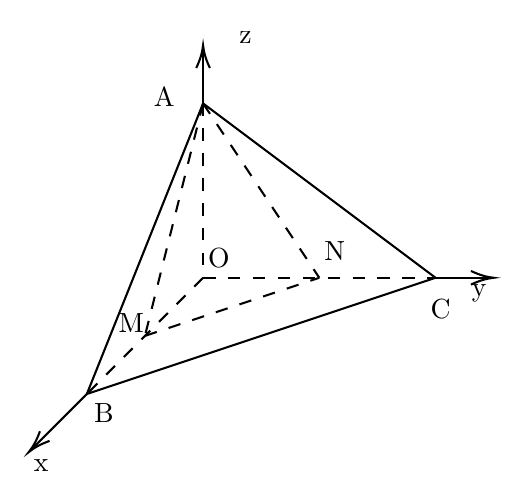
\begin{tikzpicture}[x=0.75pt,y=0.75pt,yscale=-1,xscale=1]
			%uncomment if require: \path (0,300); %set diagram left start at 0, and has height of 300
			
			%Straight Lines [id:da3679447504076472] 
			\draw  [dash pattern={on 4.5pt off 4.5pt}]  (252,140) -- (364,140) ;
			%Straight Lines [id:da13962597702284096] 
			\draw  [dash pattern={on 4.5pt off 4.5pt}]  (252,140) -- (196,196) ;
			%Straight Lines [id:da8580092790638094] 
			\draw  [dash pattern={on 4.5pt off 4.5pt}]  (252,56) -- (252,140) ;
			%Straight Lines [id:da7130062908773143] 
			\draw    (252,56) -- (196,196) ;
			%Straight Lines [id:da012778923343735649] 
			\draw    (252,56) -- (364,140) ;
			%Straight Lines [id:da3173437648870021] 
			\draw    (196,196) -- (364,140) ;
			%Straight Lines [id:da528126976168177] 
			\draw  [dash pattern={on 4.5pt off 4.5pt}]  (224,168) -- (308,140) ;
			%Straight Lines [id:da44405621585220234] 
			\draw  [dash pattern={on 4.5pt off 4.5pt}]  (252,56) -- (308,140) ;
			%Straight Lines [id:da4474952587057264] 
			\draw  [dash pattern={on 4.5pt off 4.5pt}]  (252,56) -- (224,168) ;
			%Straight Lines [id:da6666103459826491] 
			\draw    (252,56) -- (252,30) ;
			\draw [shift={(252,28)}, rotate = 90] [color={rgb, 255:red, 0; green, 0; blue, 0 }  ][line width=0.75]    (10.93,-3.29) .. controls (6.95,-1.4) and (3.31,-0.3) .. (0,0) .. controls (3.31,0.3) and (6.95,1.4) .. (10.93,3.29)   ;
			%Straight Lines [id:da6450164393512425] 
			\draw    (364,140) -- (390,140) ;
			\draw [shift={(392,140)}, rotate = 180] [color={rgb, 255:red, 0; green, 0; blue, 0 }  ][line width=0.75]    (10.93,-3.29) .. controls (6.95,-1.4) and (3.31,-0.3) .. (0,0) .. controls (3.31,0.3) and (6.95,1.4) .. (10.93,3.29)   ;
			%Straight Lines [id:da9897161761780247] 
			\draw    (196,196) -- (169.41,222.59) ;
			\draw [shift={(168,224)}, rotate = 315] [color={rgb, 255:red, 0; green, 0; blue, 0 }  ][line width=0.75]    (10.93,-3.29) .. controls (6.95,-1.4) and (3.31,-0.3) .. (0,0) .. controls (3.31,0.3) and (6.95,1.4) .. (10.93,3.29)   ;
			
			
			\draw (169,226) node [anchor=north west][inner sep=0.75pt]   [align=left] {x};
			
			\draw (380,142) node [anchor=north west][inner sep=0.75pt]   [align=left] {y};
			
			\draw (268,20) node [anchor=north west][inner sep=0.75pt]   [align=left] {z};
			
			\draw (226.8,46.8) node [anchor=north west][inner sep=0.75pt]   [align=left] {A};
			
			\draw (198,199) node [anchor=north west][inner sep=0.75pt]   [align=left] {B};
			
			\draw (360.2,149) node [anchor=north west][inner sep=0.75pt]   [align=left] {C};
			
			\draw (253,124.6) node [anchor=north west][inner sep=0.75pt]   [align=left] {O};
			
			\draw (209.8,155.6) node [anchor=north west][inner sep=0.75pt]   [align=left] {M};
			
			\draw (309,121) node [anchor=north west][inner sep=0.75pt]   [align=left] {N};
			
			
		\end{tikzpicture}
	\end{center}	
	\shortans{$0{,}9$}
	\loigiai{Chọn hệ trục tọa độ Oxyz như hình vẽ.
		
		\begin{center}
			
			\tikzset{every picture/.style={line width=0.75pt}} %set default line width to 0.75pt        
			
			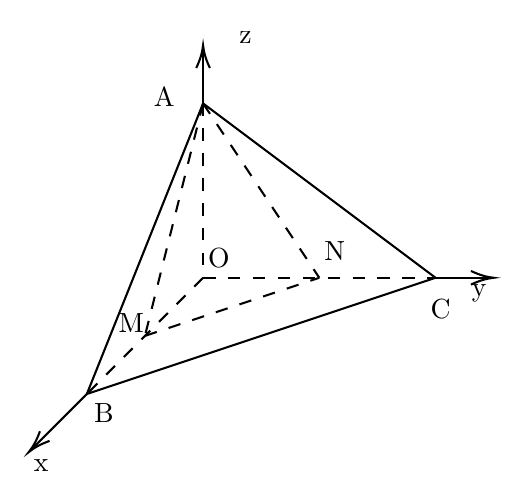
\begin{tikzpicture}[x=0.75pt,y=0.75pt,yscale=-1,xscale=1]
				
				
				%Straight Lines [id:da3679447504076472] 
				\draw  [dash pattern={on 4.5pt off 4.5pt}]  (252,140) -- (364,140) ;
				%Straight Lines [id:da13962597702284096] 
				\draw  [dash pattern={on 4.5pt off 4.5pt}]  (252,140) -- (196,196) ;
				%Straight Lines [id:da8580092790638094] 
				\draw  [dash pattern={on 4.5pt off 4.5pt}]  (252,56) -- (252,140) ;
				%Straight Lines [id:da7130062908773143] 
				\draw    (252,56) -- (196,196) ;
				%Straight Lines [id:da012778923343735649] 
				\draw    (252,56) -- (364,140) ;
				%Straight Lines [id:da3173437648870021] 
				\draw    (196,196) -- (364,140) ;
				%Straight Lines [id:da528126976168177] 
				\draw  [dash pattern={on 4.5pt off 4.5pt}]  (224,168) -- (308,140) ;
				%Straight Lines [id:da44405621585220234] 
				\draw  [dash pattern={on 4.5pt off 4.5pt}]  (252,56) -- (308,140) ;
				%Straight Lines [id:da4474952587057264] 
				\draw  [dash pattern={on 4.5pt off 4.5pt}]  (252,56) -- (224,168) ;
				%Straight Lines [id:da6666103459826491] 
				\draw    (252,56) -- (252,30) ;
				\draw [shift={(252,28)}, rotate = 90] [color={rgb, 255:red, 0; green, 0; blue, 0 }  ][line width=0.75]    (10.93,-3.29) .. controls (6.95,-1.4) and (3.31,-0.3) .. (0,0) .. controls (3.31,0.3) and (6.95,1.4) .. (10.93,3.29)   ;
				%Straight Lines [id:da6450164393512425] 
				\draw    (364,140) -- (390,140) ;
				\draw [shift={(392,140)}, rotate = 180] [color={rgb, 255:red, 0; green, 0; blue, 0 }  ][line width=0.75]    (10.93,-3.29) .. controls (6.95,-1.4) and (3.31,-0.3) .. (0,0) .. controls (3.31,0.3) and (6.95,1.4) .. (10.93,3.29)   ;
				%Straight Lines [id:da9897161761780247] 
				\draw    (196,196) -- (169.41,222.59) ;
				\draw [shift={(168,224)}, rotate = 315] [color={rgb, 255:red, 0; green, 0; blue, 0 }  ][line width=0.75]    (10.93,-3.29) .. controls (6.95,-1.4) and (3.31,-0.3) .. (0,0) .. controls (3.31,0.3) and (6.95,1.4) .. (10.93,3.29)   ;
				
				
				\draw (169,226) node [anchor=north west][inner sep=0.75pt]   [align=left] {x};
				
				\draw (380,142) node [anchor=north west][inner sep=0.75pt]   [align=left] {y};
				
				\draw (268,20) node [anchor=north west][inner sep=0.75pt]   [align=left] {z};
				
				\draw (226.8,46.8) node [anchor=north west][inner sep=0.75pt]   [align=left] {A};
				
				\draw (198,199) node [anchor=north west][inner sep=0.75pt]   [align=left] {B};
				
				\draw (360.2,149) node [anchor=north west][inner sep=0.75pt]   [align=left] {C};
				
				\draw (253,124.6) node [anchor=north west][inner sep=0.75pt]   [align=left] {O};
				
				\draw (209.8,155.6) node [anchor=north west][inner sep=0.75pt]   [align=left] {M};
				
				\draw (309,121) node [anchor=north west][inner sep=0.75pt]   [align=left] {N};
				
				
			\end{tikzpicture}
		\end{center}
		Ta có $O(0 ; 0 ; 0), A \in {Oz}, B \in O x, C \in O y$ sao cho $A O=5, OB=2, OC=4\Rightarrow A(0 ; 0 ; 5), B(2 ; 0 ; 0), C(0 ; 4 ; 0)$. $M$ là trung điểm $OB$ nên $M(1 ; 0 ; 0)$. $N$ là trung điểm $OC$ nên $N(0 ; 2 ; 0)$.\\
		Phương trình mặt phẳng $(AMN)$ qua $A$ và có véc-tơ pháp tuyến $[\overrightarrow{AM},\overrightarrow{AN}]=(10;5;2)$ là $10x + 5y + 2z - 10 = 0$.\\
		Ta có $\mathrm{d}(B;(AMN))=\mathrm{d}(O;(AMN))=\dfrac{10}{\sqrt{129}}\approx 0{,}9$.
		
	}
\end{ex}

\begin{ex}%[2H2V2-6]
	Cho hình chóp $S.ABCD$ đáy là hình thang vuông tại $A$ và $D, SA \perp(ABCD)$. Góc giữa $SB$ và mặt phẳng đáy bằng $45^{\circ}, E$ là trung điểm của $SD, AB=2a, AD = DC = a$. Chọn hệ tọa độ $Oxyz$ như hình vẽ dưới. Tính khoảng cách từ điểm $B$ đến mặt phẳng $(AEC)$ (kết quả làm tròn đến hàng phần chục).
	\begin{center}	
		
		\tikzset{every picture/.style={line width=0.75pt}} %set default line width to 0.75pt        
		
		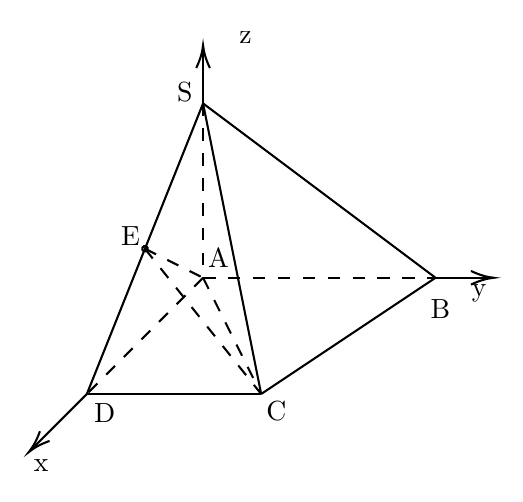
\begin{tikzpicture}[x=0.75pt,y=0.75pt,yscale=-1,xscale=1]
			%uncomment if require: \path (0,300); %set diagram left start at 0, and has height of 300
			
			%Straight Lines [id:da8913682824234928] 
			\draw  [dash pattern={on 4.5pt off 4.5pt}]  (252,140) -- (364,140) ;
			%Straight Lines [id:da039948733048584595] 
			\draw  [dash pattern={on 4.5pt off 4.5pt}]  (252,140) -- (196,196) ;
			%Straight Lines [id:da6718633500675624] 
			\draw  [dash pattern={on 4.5pt off 4.5pt}]  (252,56) -- (252,140) ;
			%Straight Lines [id:da9759242944770992] 
			\draw    (252,56) -- (196,196) ;
			\draw [shift={(224,126)}, rotate = 111.8] [color={rgb, 255:red, 0; green, 0; blue, 0 }  ][line width=0.75]      (0, 0) circle [x radius= 1.34, y radius= 1.34]   ;
			%Straight Lines [id:da563221306551871] 
			\draw    (252,56) -- (364,140) ;
			%Straight Lines [id:da15516892739193677] 
			\draw    (280,196) -- (364,140) ;
			%Straight Lines [id:da7881469638756575] 
			\draw    (252,56) -- (252,30) ;
			\draw [shift={(252,28)}, rotate = 90] [color={rgb, 255:red, 0; green, 0; blue, 0 }  ][line width=0.75]    (10.93,-3.29) .. controls (6.95,-1.4) and (3.31,-0.3) .. (0,0) .. controls (3.31,0.3) and (6.95,1.4) .. (10.93,3.29)   ;
			%Straight Lines [id:da6714011604516419] 
			\draw    (364,140) -- (390,140) ;
			\draw [shift={(392,140)}, rotate = 180] [color={rgb, 255:red, 0; green, 0; blue, 0 }  ][line width=0.75]    (10.93,-3.29) .. controls (6.95,-1.4) and (3.31,-0.3) .. (0,0) .. controls (3.31,0.3) and (6.95,1.4) .. (10.93,3.29)   ;
			%Straight Lines [id:da5385347511589023] 
			\draw    (196,196) -- (169.41,222.59) ;
			\draw [shift={(168,224)}, rotate = 315] [color={rgb, 255:red, 0; green, 0; blue, 0 }  ][line width=0.75]    (10.93,-3.29) .. controls (6.95,-1.4) and (3.31,-0.3) .. (0,0) .. controls (3.31,0.3) and (6.95,1.4) .. (10.93,3.29)   ;
			%Straight Lines [id:da05923631932446871] 
			\draw    (196,196) -- (280,196) ;
			%Straight Lines [id:da8592722804571848] 
			\draw    (252,56) -- (280,196) ;
			%Straight Lines [id:da802931795948812] 
			\draw  [dash pattern={on 4.5pt off 4.5pt}]  (252,140) -- (280,196) ;
			%Straight Lines [id:da4994838123991385] 
			\draw  [dash pattern={on 4.5pt off 4.5pt}]  (224,126) -- (252,140) ;
			%Straight Lines [id:da23640159060964017] 
			\draw  [dash pattern={on 4.5pt off 4.5pt}]  (224,126) -- (280,196) ;
			
			
			\draw (169,226) node [anchor=north west][inner sep=0.75pt]   [align=left] {x};
			
			\draw (380,142) node [anchor=north west][inner sep=0.75pt]   [align=left] {y};
			
			\draw (268,20) node [anchor=north west][inner sep=0.75pt]   [align=left] {z};
			
			\draw (238,44.4) node [anchor=north west][inner sep=0.75pt]   [align=left] {S};
			
			\draw (198,199) node [anchor=north west][inner sep=0.75pt]   [align=left] {D};
			
			\draw (360.2,149) node [anchor=north west][inner sep=0.75pt]   [align=left] {B};
			
			\draw (253,124.6) node [anchor=north west][inner sep=0.75pt]   [align=left] {A};
			
			\draw (281,198) node [anchor=north west][inner sep=0.75pt]   [align=left] {C};
			
			\draw (211,114) node [anchor=north west][inner sep=0.75pt]   [align=left] {E};
			
			
		\end{tikzpicture}
	\end{center}
	\shortans{$1{,}3$}
	\loigiai{Lấy $a=1$. Ta có $(SB,(ABCD))=\widehat{SBA}=45^0 \Rightarrow \triangle ASB$ vuông cân tại $A.$ Suy ra $SA=AB=2$.\\
	Ta có $A(0;0;0); S(0;0;2); C(1;1;0); B(0;2;0); D(1;0;0); E\left(\dfrac{1}{2};0;1\right)$.\\
	Phương trình mặt phẳng $(AEC)$ qua $A$ và có véc-tơ pháp tuyến $[\overrightarrow{AE}, \overrightarrow{AC}]=\left(-1;1;\dfrac{1}{2}\right)$ là $-2x + 2y + z = 0$.\\
	Khoảng cách từ điểm $B$ đến mặt phẳng $(AEC)$ là 
	$$\mathrm{d}(B,(AEC))=\dfrac{|2\cdot 2|}{\sqrt{2^2 +2^2 +1^2}}=\dfrac{4}{3}\approx 1{,}3.$$}
\end{ex}

\begin{ex}%[2H2V2-6]
	Trong không gian với hệ trục tọa độ $Oxyz$, cho bốn điểm $S(-1 ; 6 ; 2), A(0 ; 0 ; 6),\\ B(0 ; 3 ; 0)$, $C(-2 ; 0 ; 0)$. Gọi $H$ là chân đường cao vẽ từ $S$ của tứ diện $S.ABC$. Giả sử phương trình mặt phẳng đi qua ba điểm $S,B,H$ có dạng $x+by+cz+d=0$ với $b,c,d \in \mathbb{Z}$. Tính $b+c+d.$
	\shortans{$-17$}
	\loigiai{Phương trình mặt phẳng $(ABC): \dfrac{x}{-2}+\dfrac{y}{3}+\dfrac{z}{6}=1 \Leftrightarrow-3 x+2 y+z-6=0$. \\
	$H$ là chân đường cao vẽ từ $S$ của tứ diện $S.ABC$ nên $H$ là hình chiếu vuông góc của $S$ lên mặt phẳng $(A B C) \Rightarrow H\left(\dfrac{19}{14} ; \dfrac{31}{7} ; \dfrac{17}{14}\right)$.\\
	Mặt phẳng $(SBH)$ qua $B(0;3;0)$ và có véc-tơ pháp tuyến $$[\overrightarrow{BH}, \overrightarrow{SB}]=\left(\dfrac{11}{14} ; \dfrac{55}{14} ;-\dfrac{11}{2}\right)=\dfrac{11}{14}(1 ; 5 ;-7).$$
	Phương trình mặt phẳng $(SBH)$ là $ x+5(y-3)-7 z=0\\ \Leftrightarrow x+5 y-7 z-15=0$. Ta có $b+c+d =-17.$
	}
\end{ex}
\begin{ex}%[2H2V2-6]
	Trong KG $Oxyz$, cho hình chóp $S.ABCD$, đáy $ABCD$ là hình chữ nhật. Biết $A(0 ; 0 ; 0), D(2 ; 0 ; 0), B(0 ; 4 ; 0), S(0 ; 0 ; 4)$. Gọi $M$ là trung điểm của $SB$ và $G$ là trọng tâm của tam giác $SCD$. Tính khoảng cách từ điểm $B$ đến mặt phẳng $(AMG)$. Kết quả làm tròn đến hàng phần chục.
	\shortans{$2{,}8$}
	\loigiai{
		\begin{center}
			\tikzset{every picture/.style={line width=0.75pt}} %set default line width to 0.75pt        
			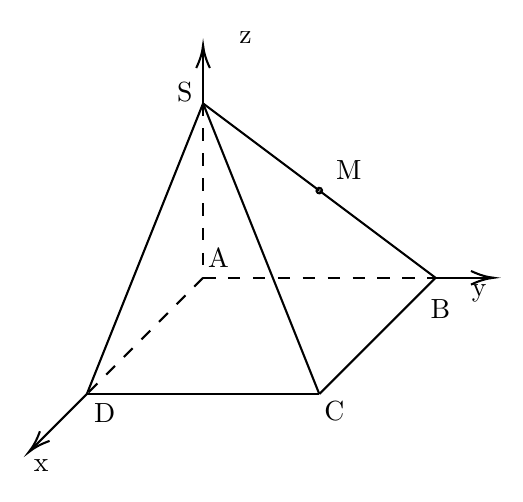
\begin{tikzpicture}[x=0.75pt,y=0.75pt,yscale=-1,xscale=1]
				%uncomment if require: \path (0,300); %set diagram left start at 0, and has height of 300
				
				%Straight Lines [id:da8697087570722153] 
				\draw  [dash pattern={on 4.5pt off 4.5pt}]  (252,140) -- (364,140) ;
				%Straight Lines [id:da4072889759548881] 
				\draw  [dash pattern={on 4.5pt off 4.5pt}]  (252,140) -- (196,196) ;
				%Straight Lines [id:da5044623873055065] 
				\draw  [dash pattern={on 4.5pt off 4.5pt}]  (252,56) -- (252,140) ;
				%Straight Lines [id:da6764918883827946] 
				\draw    (252,56) -- (196,196) ;
				%Straight Lines [id:da4329647923634008] 
				\draw    (252,56) -- (308,98) ;
				%Straight Lines [id:da011038461362765872] 
				\draw    (308.27,98.2) -- (364,140) ;
				\draw [shift={(308,98)}, rotate = 36.87] [color={rgb, 255:red, 0; green, 0; blue, 0 }  ][line width=0.75]      (0, 0) circle [x radius= 1.34, y radius= 1.34]   ;
				%Straight Lines [id:da5196781175343534] 
				\draw    (308,196) -- (364,140) ;
				%Straight Lines [id:da3160409919917737] 
				\draw    (252,56) -- (252,30) ;
				\draw [shift={(252,28)}, rotate = 90] [color={rgb, 255:red, 0; green, 0; blue, 0 }  ][line width=0.75]    (10.93,-3.29) .. controls (6.95,-1.4) and (3.31,-0.3) .. (0,0) .. controls (3.31,0.3) and (6.95,1.4) .. (10.93,3.29)   ;
				%Straight Lines [id:da9102255389540188] 
				\draw    (364,140) -- (390,140) ;
				\draw [shift={(392,140)}, rotate = 180] [color={rgb, 255:red, 0; green, 0; blue, 0 }  ][line width=0.75]    (10.93,-3.29) .. controls (6.95,-1.4) and (3.31,-0.3) .. (0,0) .. controls (3.31,0.3) and (6.95,1.4) .. (10.93,3.29)   ;
				%Straight Lines [id:da3969763351140396] 
				\draw    (196,196) -- (169.41,222.59) ;
				\draw [shift={(168,224)}, rotate = 315] [color={rgb, 255:red, 0; green, 0; blue, 0 }  ][line width=0.75]    (10.93,-3.29) .. controls (6.95,-1.4) and (3.31,-0.3) .. (0,0) .. controls (3.31,0.3) and (6.95,1.4) .. (10.93,3.29)   ;
				%Straight Lines [id:da06997294598351322] 
				\draw    (196,196) -- (308,196) ;
				%Straight Lines [id:da06948427828035464] 
				\draw    (252,56) -- (308,196) ;
				
				
				\draw (169,226) node [anchor=north west][inner sep=0.75pt]   [align=left] {x};
				
				\draw (380,142) node [anchor=north west][inner sep=0.75pt]   [align=left] {y};
				
				\draw (268,20) node [anchor=north west][inner sep=0.75pt]   [align=left] {z};
				
				\draw (238,44.4) node [anchor=north west][inner sep=0.75pt]   [align=left] {S};
				
				\draw (198,199) node [anchor=north west][inner sep=0.75pt]   [align=left] {D};
				
				\draw (360.2,149) node [anchor=north west][inner sep=0.75pt]   [align=left] {B};
				
				\draw (253,124.6) node [anchor=north west][inner sep=0.75pt]   [align=left] {A};
				
				\draw (309,198) node [anchor=north west][inner sep=0.75pt]   [align=left] {C};
				
				\draw (314.6,82) node [anchor=north west][inner sep=0.75pt]   [align=left] {M};
			\end{tikzpicture}
		\end{center}
		Chọn hệ trục tọa độ như hình vẽ. Ta có $A(0 ; 0 ; 0), D(2 ; 0 ; 0), B(0 ; 4 ; 0), S(0 ; 0 ; 4)$.\\
		$M$ là trung điểm của $S B \Rightarrow M(0 ; 2 ; 2)$.\\
		Tứ giác $A B C D$ là hình chữ nhật nên $\left\{\begin{array}{l}x_{A}+x_{C}=x_{B}+x_{D} \\ y_{A}+y_{C}=y_{B}+y_{D} \\ z_{A}+z_{C}=z_{B}+z_{D}\end{array} \Rightarrow\left\{\begin{array}{l}x_{C}=2 \\ y_{C}=4 \\ z_{C}=0\end{array} \Rightarrow C(2 ; 4 ; 0)\right.\right.$.\\
		$G$ là trọng tâm của tam giác $S C D \Rightarrow G\left(\dfrac{4}{3}; \dfrac{4}{3} ; \dfrac{4}{3}\right)$.\\
		Phương trình mặt phẳng $(AMG)$ qua $A$ và có véc-tơ pháp tuyến $[\overrightarrow{AM},\overrightarrow{AG}]=\left(0;\dfrac{-8}{3};\dfrac{8}{3} \right)$ là $y-z=0.$\\
		Khoảng cách từ điểm B đến mặt phẳng $(AMG)$ là $\mathrm{d}(B,(AMG))= \dfrac{|4|}{\sqrt{1^2+1^2}}=\dfrac{4}{\sqrt{2}}\approx 2{,}8$.
	}
\end{ex}

\begin{ex}%[2H2V2-6]
	Cho hình hộp chữ nhật $ABCD \cdot A'B'C'D'$ có các kích thước $AB=4, AD=3, AA'=5$. Gọi $G$ là trọng tâm của tam giác $ACB'$. Gọi $m$ là khoảng cách từ điểm $G$ đến mặt phẳng $\left(AB'C\right)$ và $n$ là khoảng cách giữa hai mặt phẳng $(AB'D')$ và $(CB'D')$. Tính $m+n$.
	\shortans{$0$}
	\loigiai{
	\begin{center}
	\tikzset{every picture/.style={line width=0.75pt}} %set default line width to 0.75pt        
	\begin{tikzpicture}[x=0.75pt,y=0.75pt,yscale=-1,xscale=1]
	%Straight Lines [id:da09989011048457908] 
	\draw    (250,400) -- (250,327) ;
	\draw [shift={(250,325)}, rotate = 90] [color={rgb, 255:red, 0; green, 0; blue, 0 }  ][line width=0.75]    (10.93,-3.29) .. controls (6.95,-1.4) and (3.31,-0.3) .. (0,0) .. controls (3.31,0.3) and (6.95,1.4) .. (10.93,3.29)   ;
	%Straight Lines [id:da5887885003342179] 
	\draw    (175,575) -- (375,575) ;
	%Straight Lines [id:da38181530618442316] 
	\draw    (375,575) -- (450,500) ;
	%Straight Lines [id:da5520368192051237] 
	\draw    (250,400) -- (175,475) ;
	%Straight Lines [id:da857881333421624] 
	\draw    (175,475) -- (175,575) ;
	%Straight Lines [id:da1055531864002952] 
	\draw    (175,475) -- (375,475) ;
	%Straight Lines [id:da9921967082690255] 
	\draw    (375,475) -- (375,575) ;
	%Straight Lines [id:da830188535856651] 
	\draw    (375,475) -- (450,400) ;
	%Straight Lines [id:da8543854930333936] 
	\draw    (250,400) -- (450,400) ;
	%Straight Lines [id:da010540648916782303] 
	\draw    (450,400) -- (450,500) ;
	%Straight Lines [id:da5916479203423954] 
	\draw  [dash pattern={on 4.5pt off 4.5pt}]  (250,500) -- (175,575) ;
	%Straight Lines [id:da3953089475850997] 
	\draw    (175,575) -- (126.41,623.59) ;
	\draw [shift={(125,625)}, rotate = 315] [color={rgb, 255:red, 0; green, 0; blue, 0 }  ][line width=0.75]    (10.93,-3.29) .. controls (6.95,-1.4) and (3.31,-0.3) .. (0,0) .. controls (3.31,0.3) and (6.95,1.4) .. (10.93,3.29)   ;
	%Straight Lines [id:da9157272689802225] 
	\draw  [dash pattern={on 4.5pt off 4.5pt}]  (250,500) -- (450,500) ;
	%Straight Lines [id:da9303391433588712] 
	\draw    (450,500) -- (523,500) ;
	\draw [shift={(525,500)}, rotate = 180] [color={rgb, 255:red, 0; green, 0; blue, 0 }  ][line width=0.75]    (10.93,-3.29) .. controls (6.95,-1.4) and (3.31,-0.3) .. (0,0) .. controls (3.31,0.3) and (6.95,1.4) .. (10.93,3.29)   ;
	%Straight Lines [id:da1786416964548232] 
	\draw  [dash pattern={on 4.5pt off 4.5pt}]  (250,400) -- (250,500) ;
	\draw (177,478) node [anchor=north west][inner sep=0.75pt]   [align=left] {D'};
	
	\draw (252,403) node [anchor=north west][inner sep=0.75pt]   [align=left] {A'};
	
	\draw (452,403) node [anchor=north west][inner sep=0.75pt]   [align=left] {B'};
	
	\draw (376,481) node [anchor=north west][inner sep=0.75pt]   [align=left] {C'};
	
	\draw (177,578) node [anchor=north west][inner sep=0.75pt]   [align=left] {D};
	
	\draw (252,503) node [anchor=north west][inner sep=0.75pt]   [align=left] {A};
	
	\draw (452,503) node [anchor=north west][inner sep=0.75pt]   [align=left] {B};
	
	\draw (377,578) node [anchor=north west][inner sep=0.75pt]   [align=left] {C};
	
	\draw (513,518) node [anchor=north west][inner sep=0.75pt]   [align=left] {x};
	
	\draw (140,620) node [anchor=north west][inner sep=0.75pt]   [align=left] {y};
	
	\draw (263,331) node [anchor=north west][inner sep=0.75pt]   [align=left] {z};
	\end{tikzpicture}
\end{center}			
		Chọn hệ trục tọa độ như hình vẽ. Ta có $A(0;0 ; 0), C(4 ; 3 ; 0), B'(4 ; 0 ; 5), B(4 ; 0 ; 0); D'(0;3;5).$ $G$ là trọng tâm của tam giác $ACB' \Rightarrow G\left(\dfrac{8}{3} ; 1 ; \dfrac{5}{3}\right).$\\
		Vì $G \in (ACB')$ nên $\mathrm{d}(G, (ACB'))=0.$\\
		Vì hai mặt phẳng $(AB'D')$ và $(CB'D')$ cắt nhau nên khoảng cách của chúng  bằng $0.$ \\
		Vậy $m+n=0$.}
\end{ex}
\Closesolutionfile{ans}
% \indapan{6}{ans/ans-0-B15-KQ}

